\section{The normal linear model}

\subsection{Multivariate normal distribution}
Let $X = (X_1, \dots, X_n)$ be a vector of random variables.
Then we define
\begin{align*}
	\expect{X} = \begin{pmatrix}
		\expect{X_1} \\
		\vdots       \\
		\expect{X_n}
	\end{pmatrix};\quad \Var{X} = V_{ij} = \expect{\qty(X_i - \expect{X_i})\qty(X_j - \expect{X_j})}
\end{align*}
The familiar linearity results are
\begin{align*}
	\expect{AX+b} = A\expect{X} + b;\quad \Var{AX + b} = A \Var{X} A^\tran
\end{align*}
where $A \in \mathbb R^{k \times n}, b \in \mathbb R^k$ are constant.

\begin{definition}[Multivariate Normal Distribution (MVN)]
	We say that $X$ has a \vocab{multivariate normal distribution} if, for any fixed $t \in \mathbb R^n$, $t^\tran X$ is normal.
\end{definition}

\begin{proposition}
	Let $X$ be multivariate normal.
	Then $AX+b$ is multivariate normal, where $A \in \mathbb R^{k \times n}, b \in \mathbb R^k$ are constant.
\end{proposition}

\begin{proof}
	Let $t \in \mathbb R^k$.
	Then,
	\begin{align*}
		t^\tran (Ax+b) = \underbrace{(A^\tran t)^\tran X}_{\sim N(\mu, \sigma^2)} + t^\tran b
	\end{align*}
	which is the sum of a normal random variable and a constant.
	So this is $N(\mu + t^\tran b, \sigma^2)$.
\end{proof}

\begin{proposition}
	A MVN is fully specified by its mean and covariance matrix.
\end{proposition}

\begin{proof}
	Let $X_1, X_2$ be MVN with the same mean $\mu$ and the same covariance matrix $\Sigma$.
	We will show that these two random variables have the same moment generating function, and hence the same distribution.
	\begin{align*}
		M_{X_1}(t) = \expect{ e^{1 \cdot t^\tran X_1} }
	\end{align*}
	Note that $t^\tran X_1$ is univariate normal.
	Hence, this is equal to
	\begin{align*}
		M_{X_1}(t) = \exp(1 \cdot \expect{t^\tran X_1} + \frac{1}{2} \Var{t^\tran X_1} \cdot 1^2) = \exp(t^\tran \mu + \frac{1}{2} t^\tran \Sigma t)
	\end{align*}
	This depends only on $\mu$ and $\Sigma$, and we obtain the same moment generating function for $X_2$.
\end{proof}

\subsection{Orthogonal projections}
\begin{definition}[Orthogonal Projection]
	A matrix $P \in \mathbb R^{n \times n}$ is an \vocab{orthogonal projection} onto its column space $\mathrm{col}(P)$ if, for all $v \in \mathrm{col}(P)$, we have $Pv = v$, and for all $w \in \mathrm{col}(P)^\perp$, we have $Pw = 0$.
\end{definition}

\begin{proposition}
	$P$ is an orthogonal projection iff it is idempotent and symmetric.
\end{proposition}

\begin{proof}
	$(\Longleftarrow)$: Let $v \in \mathrm{col}(P)$, so $v = Pa$ for some $a \in \mathbb R^n$.
	Then, $Pv = PPa = Pa$ as $P$ idempotent. \\
	Now, let $w \in \mathrm{col}(P)^\perp$.
	By definition, $P^\tran w = 0$.
	By symmetry, $Pw = 0$.

	$(\implies)$: Any vector $a \in \mathbb R^n$ can be uniquely written as $a = v + w$ where $v \in \mathrm{col}(P)$ and $w \in \mathrm{col}(P)^\perp$.
	Then $PPa = PPv + PPw = Pv = P(v+w) = Pa$.
	As this holds for all $a$, we have that $P$ is idempotent. \\
	Let $u_1, u_2 \in \mathbb R^n$, and note $(P u_1) \cdot ((I-P) u_2) = 0$, as $P u_1 \in \mathrm{col}(P)$ and $(I-P) u_2 \in \mathrm{col}(P)^\perp$.
	We have $u_1^\tran P^\tran (I-P) u_2 = 0$.
	Since this holds for all $u_1, u_2$, $P^\tran (I-P) = 0$ so $P^\tran = P^\tran P$.
	Note that $P^\tran P$ is symmetric, so $P^\tran$ is symmetric, and hence $P$ is symmetric.
\end{proof}

\begin{corollary}
	Let $P$ be an orthogonal projection matrix.
	Then $I-P$ is also an orthogonal projection matrix.
\end{corollary}

\begin{proof}
	Clearly, if $P$ is symmetric, so is $I-P$, so it suffices to prove idempotence.
	We have $(I-P)(I-P) = I - 2P + P^2 = I - 2P + P = I - P$ as required.
\end{proof}

\begin{proposition}
	If $P \in \mathbb{R}^{n \times n}$ is an orthogonal projection, then $P = UU^\tran$\footnote{If $k = \rank P$ then $U \in \mathbb{R}^{n \times k}$} where the columns of $U$ are an orthonormal basis for the column space of $P$.
\end{proposition}

\begin{proof}
	First, we show that $UU^\tran$ is an orthogonal projection.
	This is clearly symmetric.
	It is idempotent: $U U^\tran U U^\tran = U U^\tran$ since $U^\tran U = I$, as the columns of $U$ form an orthonormal basis for the column space of $P$.

	Further, the column space of $P$ is exactly the column space of $U U^\tran$, so $P = U U^\tran$.
\end{proof}

\begin{proposition}
	The rank of an orthogonal projection matrix is equal to its trace.
\end{proposition}

\begin{proof}
	The rank is the dimension of the column space, which is $\rank P = \rank(U^\tran U)$, $U^\tran U = I_k$ where $k = \rank P$ so $\rank (U^\tran U) = k = \tr(U^\tran U) = \tr(U U^\tran) = \tr P$.
\end{proof}

\begin{theorem} \label{thm:6.1}
	Let $X$ be MVN, where $X \sim N(0,\sigma^2 I)$, and let $P$ be an orthogonal projection.
	Then
	\begin{enumerate}
		\item $PX \sim N(0,\sigma^2 P)$, $(I-P)X \sim N(0,\sigma^2(I-P))$ and these two random variables are independent;
		\item $\frac{\norm{PX}^2}{\sigma^2} \sim \chi^2_{\rank P}$.
	\end{enumerate}
\end{theorem}

\begin{proof}
	The vector $(P, I-P)^\tran X$ is multivariate normal, since it is a linear function of $X$.
	This distribution is fully specified by its mean and variance.
	\begin{align*}
		\expect{\begin{pmatrix}
				PX \\
				(I-P)X
			\end{pmatrix}} = \begin{pmatrix}
			P \\
			I-P
		\end{pmatrix} \expect{X} = 0
	\end{align*}
	Further,
	\begin{align*}
		\Var{\begin{pmatrix}
				PX \\
				(I-P)X
			\end{pmatrix}} &= \begin{pmatrix}
			P \\
			I - P
		\end{pmatrix} \sigma^2 I \begin{pmatrix}
			P \\
			I - P
		\end{pmatrix}^\tran \\
		&= \sigma^2 \begin{pmatrix}
			P^2    & P(I-P)  \\
			P(I-P) & (I-P)^2
		\end{pmatrix} \\
		&= \sigma^2 \begin{pmatrix}
			P & 0   \\
			0 & I-P
		\end{pmatrix}\footnote{$P(I - P) = P - P^2 = P - P = 0$ as $P$ idemptotent.}
	\end{align*}
	Now we must show that the variables $PX, (I-P)X$ are independent.
	Let $Z \sim N(0,\sigma^2 P), Z' \sim N(0,\sigma^2(I-P))$ be independent.
	Then we can see that $(Z, Z')^\tran$ is multivariate normal with
	\begin{align*}
		\mu = 0;\quad \Sigma = \sigma^2 \begin{pmatrix}
			P & 0     \\
			0 & I - P
		\end{pmatrix}
	\end{align*}
	Hence $(PX, (1-P)X)^\tran$ is equal in distribution to $(Z, Z')^\tran$.
	So $PX$ is independent of $(I-P)X$. \\

	We must show that $\frac{\norm{PX}^2}{\sigma^2} \sim \chi^2_{\rank P}$.
	Note that
	\begin{align*}
		\frac{\norm{PX}^2}{\sigma^2} = \frac{X^\tran P^\tran P X}{\sigma^2} = \frac{X^\tran \qty(U U^\tran)^\tran U U^\tran X}{\sigma^2} = \frac{X^\tran U U^\tran X}{\sigma^2}
	\end{align*}
	The columns of $U$ form an orthogonal basis of the columns of $P$ so
	\begin{align*}
		\frac{\norm{PX}^2}{\sigma^2} &= \frac{\norm{U^\tran X}^2}{\sigma^2} \\
		&= \sum_{i = 1}^{\rank P} \frac{(U^\tran X)^2_i}{\sigma^2}.
	\end{align*} 
	Note, $U^\tran X \sim N(0,\sigma^2 U^\tran U) = N(0,\sigma^2 I_{\rank P})$.
	\begin{align*}
		\Var{U^\tran X} &= U^\tran \Var X U \\
		&= \sigma^2 U^\tran U \\
		&= \sigma^2 I. 
	\end{align*} 
	So
	\begin{align*}
		\frac{(U^\tran X)_i}{\sigma} \overset{\text{iid}}{\sim} N(0, 1)
	\end{align*}
	for $i = 1, \dots, \rank P$.
	Hence
	\begin{align*}
		\frac{\norm{PX}^2}{\sigma^2} = \sum_{i=1}^{\rank P} \qty(\frac{(U^\tran X)_i}{\sigma})^2 \sim \chi^2_{\rank P}
	\end{align*}
\end{proof}

\begin{theorem}
	Let $X_1, \dots, X_n \overset{\text{iid}}{\sim} N(\mu,\sigma^2)$ for some unknown $\mu \in \mathbb R$ and $\sigma^2 > 0$.
	The maximum likelihood estimators for $\mu$ and $\sigma$ are
	\begin{align*}
		\hat \mu = \overline X = \frac{1}{n} \sum_i X_i;\quad \hat \sigma^2 = \frac{S_{xx}}{n} = \frac{\sum_i \qty(X_i - \overline X)^2}{n}
	\end{align*}
	Further,
	\begin{enumerate}
		\item $\overline X \sim N\qty(\mu, \frac{\sigma^2}{n})$;
		\item $\frac{S_{xx}}{\sigma^2} \sim \chi^2_{n-1}$;
		\item $\overline X, S_{xx}$ are independent.
	\end{enumerate}
\end{theorem}

\begin{proof}
	We have proved the first statement before.

	Let $P$ be the square $n \times n$ matrix with all entries $\frac{1}{n}$.
	This is an orthogonal projection matrix, as it is symmetric and idempotent.
	Note that
	\begin{align*}
		PX = \begin{pmatrix}
			\overline X \\
			\vdots      \\
			\overline X
		\end{pmatrix}
	\end{align*}
	We will write the observations $X$ as
	\begin{align*}
		X = \underbrace{\begin{pmatrix}
				\mu    \\
				\vdots \\
				\mu
			\end{pmatrix}}_{M} + \varepsilon;\quad \varepsilon \sim N(0,\sigma^2 I)
	\end{align*}
	Note that $\overline X$ is a function of $P \varepsilon$, since $\overline X = (PX)_1 = (PM + P\varepsilon)_1$.
	Further,
	\begin{align*}
		S_{xx} = \sum_i \qty(X_i - \overline X)^2 = \norm{X - PX}^2 = \norm{(I-P)X}^2 = \norm{(I-P)\varepsilon}^2
	\end{align*}
	Hence $S_{xx}$ is a function of $(I-P)\varepsilon$.
	By the previous theorem, $P\varepsilon$ and $(I-P)\varepsilon$ are independent, so $\overline X$ and $S_{xx}$ are independent.

	Since $I-P$ is a projection with rank equal to its trace $n-1$, we apply the previous theorem to obtain
	\begin{align*}
		\frac{S_{xx}}{\sigma^2} = \frac{\norm{(I-P)\varepsilon}^2}{\sigma^2} = \chi^2_{n-1}
	\end{align*}
\end{proof}

\subsection{Linear model}
Suppose we have data in pairs $(x_1, Y_1), \dots, (x_n, Y_n)$, where $Y_i \in \mathbb R, x_i \in \mathbb R^p$.
The $Y_i$ are known as the \vocab{response} variables, or the \vocab{dependent} variables.
The $x_{i1}, x_{ip}$ are the \vocab{predictors}, or \vocab{independent} variables.
We will model the expectation of the response $Y_i$ as a linear function of the predictors $(x_{i1}, \dots, x_{ip})$.
\begin{example}
	Let $Y_i$ be the number of insurance claims that driver $i$ makes in a given year, and $x_{i1}, \dots, x_{ip}$ is a set of variables about the specific driver.
	Predictors include age, the number of years they have held their license, and the number of points on their license, for instance.
\end{example}
We assume that
\begin{align*}
	Y_i = \alpha + \beta_1 x_{i1} + \dots + \beta_p x_{ip} + \varepsilon_i
\end{align*}
where $\alpha \in \mathbb R$ is an \vocab{intercept}, $\beta_i$ are the \vocab{coefficients}, and $\varepsilon$ is a \vocab{noise vector}, which is a random variable.
The intercept and coefficients are the parameters of interest.

\begin{remark}
	\begin{enumerate}
		\item We will often eliminate the intercept by making one of the predictors $x_{i1} = 1$ for all $i$, so $\beta_1$ plays the role of the intercept.
		\item Note that we can use a linear model to model nonlinear relationships.
		For example, suppose $Y_i = a + bz_i + cz_i^2 + \varepsilon_i$.
		We can rephrase this as a linear model with $x_i = (1, z_i, z_i^2)$.
		\item The coefficient $\beta_j$ can be interpreted as the effect on $Y_i$ of increasing $x_{ij}$ by one, while keeping all other predictors fixed.
		This cannot be interpreted as a causal relationship in general.
	\end{enumerate} 
\end{remark} 

\subsection{Matrix formulation}
Let
\begin{align*}
	Y = \begin{pmatrix}
		Y_1    \\
		\vdots \\
		Y_n
	\end{pmatrix};\quad X = \begin{pmatrix}
		x_{11} & \cdots & x_{1p} \\
		\vdots & \ddots & \vdots \\
		x_{n1} & \cdots & x_{np}
	\end{pmatrix};\quad \beta = \begin{pmatrix}
		\beta_1 \\
		\vdots  \\
		\beta_p
	\end{pmatrix};\quad \varepsilon = \begin{pmatrix}
		\varepsilon_1 \\
		\vdots        \\
		\varepsilon_n
	\end{pmatrix}
\end{align*}
We call $X$ the \vocab{design matrix}.
The linear model is that
\begin{align*}
	Y = X\beta + \varepsilon
\end{align*}
$X\beta$ is considered fixed.
Since $\varepsilon$ is random, this makes $Y$ into a random variable.

\subsection{Assumptions}
We make a number of \vocab{moment assumptions} on the noise vector $\varepsilon$.
This allows us to deduce more results about the linear model.
\begin{enumerate}
	\item $\expect{\varepsilon} = 0 \implies \expect{Y_i} = x_i^\tran \beta$;
	\item $\Var \varepsilon = \sigma^2 I$, which is equivalent to both $\Var \varepsilon_i = \sigma^2$ and $\Cov{\varepsilon_i, \varepsilon_j} = 0$ for all $i \neq j$.
	      This property is known as \vocab{homoscedasticity}.
\end{enumerate}
We will always assume that the design matrix $X$ has full rank $p$, or equivalently, that it has linearly independent columns.
Since $X \in \mathbb R^{n \times p}$, this requires that $n \geq p$, so we need at least as many samples as we have predictors.

\subsection{Least squares estimation}
\begin{definition}[Least Squares Estimator]
	The \vocab{least squares estimator} $\hat \beta$ minimises the \vocab{residual sum of squares}, which is
	\begin{align*}
		S(\beta) = \norm{Y-X\beta}^2 = \sum_i \qty(Y_i - x_i^\tran \beta)^2
	\end{align*}
	The term $Y_i - x_i^\tran \beta$ is called the \text{$i$th residual}.
\end{definition}

Since $S(\beta)$ is a positive definite quadratic in $\beta$, it is minimised at the stationary point.
\begin{align*}
	\eval{\pdv{S(\beta)}{\beta_k}}_{\beta = \hat \beta} = 0 \iff \forall k,\;-2\sum_{i=1}^n x_{ik} \qty(Y_i - \sum_k x_{ij} \hat \beta_j) = 0 \iff X^\tran X \hat \beta = X^\tran Y
\end{align*}

As $X$ has full column rank, $X^\tran X \in \mathbb{R}^{p \times p}$ is invertible.
\begin{align*}
	\hat \beta = (X^\tran X)^{-1} X^\tran Y
\end{align*}
This is notably a linear function of $Y$, given fixed $X$.
Note that
\begin{align*}
	\expect{\hat \beta} = (X^\tran X)^{-1} X^\tran \expect{Y} = (X^\tran X)^{-1} X^\tran X\beta = \beta
\end{align*}

So $\hat \beta$ is an unbiased estimator.
Further,
\begin{align*}
	\Var{\hat \beta} &= (X^\tran X)^{-1} X^\tran \Var Y \qty[(X^\tran X)^{-1} X^\tran]^\tran     \\
	                 &= (X^\tran X)^{-1} X^\tran \sigma^2 I \qty[(X^\tran X)^{-1} X^\tran]^\tran \\
	                 &= \sigma^2 (X^\tran X)^{-1}
\end{align*}

\begin{theorem}[Gauss-Markov theorem] \label{thm:gauss}
	Let an estimator $\beta^\star$ of $\beta$ be unbiased and a linear function of $Y$, so $\beta^\star = CY$.
	Then, for any fixed $t \in \mathbb R^p$, we have
	\begin{align*}
		\Var{t^\tran \hat \beta} \leq \Var{t^\tran \beta^\star}
	\end{align*}
	where $\hat \beta$ is the least squares estimator.
	We say that $\hat \beta$ is the best linear unbiased estimator (BLUE).
\end{theorem}

\begin{remark}
	We can think of $t \in \mathbb R^p$ as a vector of predictors for a new sample.
	Then $t^\tran \hat \beta$ is the prediction for $\expect{Y_i}$ for this new sample, using the least squares estimator.
	$t^\tran \beta^\star$ is the prediction with $\beta^\star$.
	In both cases, the prediction is unbiased.
\end{remark}

\begin{proof}
	Note that
	\begin{align*}
		\Var{t^\tran \beta^\star} - \Var{t^\tran \hat \beta} = t^\tran \qty[\Var{\beta^\star} - \Var{\hat\beta}] t
	\end{align*}
	To prove that this quantity is always non-negative, we must show that $\Var{\beta^\star} - \Var{\hat\beta}$ is positive semidefinite.
	Recall $\beta^\star = CY, \hat{\beta} = (X^\tran X)\inv X^\tran Y$ so let $A = C - (X^\tran X)^{-1} X^\tran$.
	Note that $\expect{AY} = \expect{\beta^\star} - \expect{\hat\beta} = 0$.
	Also, $\expect{AY} = A \expect{Y} = AX\beta$.
	This holds for all $\beta$, so $AX = 0$.
	Now, since $X^\tran X$ is symmetric,
	\begin{align*}
		\Var{\beta^\star} & = \Var{CY} \\
		& = \Var{(A+(X^\tran X)^{-1} X^\tran)Y} \\
		& = \qty[A+(X^\tran X)^{-1} X^\tran] \Var Y \qty[A+(X^\tran X)^{-1} X^\tran]^\tran \\
		& = \qty[A+(X^\tran X)^{-1} X^\tran] \sigma^2 I \qty[A+(X^\tran X)^{-1} X^\tran]^\tran \\
		& = \sigma^2 \qty(A A^\tran + (X^\tran X)^{-1} + \underbracket{AX(X^\tran X)^{-1} + (X^\tran X)^{-1} X^\tran A^\tran}_{AX = 0}) \\
		& = \sigma^2 AA^\tran + \Var{\hat \beta} \\
		\Var{\beta^\star} - \Var{\hat\beta} & = \sigma^2 AA^\tran
	\end{align*}
	Note that the outer product $A A^\tran$ is always positive semidefinite.
\end{proof}

\subsection{Fitted values and residuals}
\begin{definition}
	The \vocab{fitted values} are $\hat Y = X \hat \beta = X(X^\tran X)^{-1} X^\tran Y$, where $P = X (X^\tran X)^{-1} X^\tran$ is the \vocab{hat matrix}.
	The \vocab{residuals} are $Y - \hat Y = (I-P)Y$.
\end{definition}

\begin{proposition}
	$P$ is the orthogonal projection onto the column space of the design matrix.
\end{proposition}

\begin{proof}
	$P$ is clearly symmetric.
	$P$ is idempotent:
	\begin{align*}
		P^2 &= X (X^\tran X)\inv X^\tran X (X^\tran X)\inv X^\tran \\
		&= P.
	\end{align*}
	Therefore $P$ is an orthogonal projection.
	We need to show column space of $P$ is the column space of $X$. 

	If $v$ is in the column space of $X$, then $v = Xb$ for some $b$.
	Hence
	\begin{align*}
		\operatorname{col}(P) \ni Pv = X(X^\tran X)^{-1} X^\tran X b = Xb = v
	\end{align*}
	For any $a$ 
	\begin{align*}
		Pa = X(X^\tran X)^{-1} X^\tran a \in \operatorname{col}(X).
	\end{align*} 
\end{proof}

\begin{corollary}
	The fitted values are an orthogonal projection of $Y$ to the column space of $X$.
	The residuals are orthogonal to the column space, they are a projection of $Y$ onto the orthogonal of the column space of $X$. 
\end{corollary}

\begin{figure}[h] 
    \centering 
    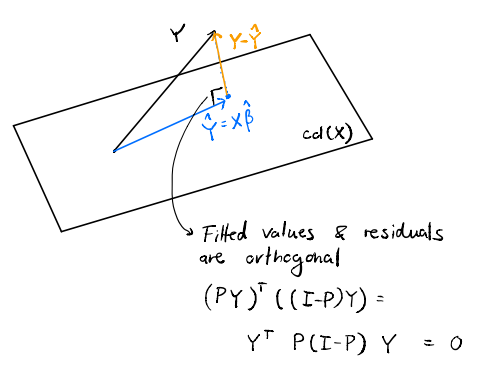
\includegraphics[height=5cm]{06-geometric} 
\end{figure}

\subsection{Normal linear model}

The normal linear model is a linear model under the assumption that $\varepsilon \sim N(0,\sigma^2 I)$, where $\sigma^2$ is unknown.
The parameters in the model are now $(\beta, \sigma^2)$.
The likelihood function in the normal linear model is
\begin{align*}
	L(\beta, \sigma^2) = f_Y(y\mid \beta,\sigma^2) = (2\pi \sigma^2)^{-\frac{n}{2}} \exp{-\frac{1}{2\sigma^2} \sum_i (Y_i - x_i^\tran \beta)^2}
\end{align*}
The log-likelihood is
\begin{align*}
	\ell(\beta,\sigma^2) = \text{constant} - \frac{n}{2}\log \sigma^2 - \frac{1}{2\sigma^2} \norm{Y-X\beta}^2
\end{align*}
To maximise this as a function of $\beta$ for any fixed $\sigma^2$, we must minimise the residual sum of squares $S(\beta) = \norm{Y-X\beta}^2$.
So $\hat \beta = (X^\tran X)^{-1} X^\tran Y$ is the maximum likelihood estimator of $\beta$.
Further, $\hat \sigma^2 = n^{-1} \norm{Y-X\hat\beta}^2 = n^{-1} \norm{\hat Y - Y}^2 = n^{-1} \norm{(I-P)Y}^2$.

\begin{theorem}
	In the normal linear model,
	\begin{enumerate}
		\item $\hat \beta \sim N(\beta,\sigma^2(X^\tran X)^{-1})$;
		\item $n\frac{\hat\sigma^2}{\sigma^2} \sim \chi^2_{n-p}$;
		\item $\hat \beta, \hat \sigma^2$ are independent.
	\end{enumerate}
\end{theorem}

\begin{proof}
	We prove each part separately.
	\begin{enumerate}
		\item We already know that $\expect{\hat \beta} = \beta$, and $\Var{\hat \beta} = \sigma^2 (X^\tran X)^{-1}$.
		      So it suffices to show that $\hat \beta$ is a MVN.
		      Since $\hat \beta = (X^\tran X)^{-1} X^\tran Y$, it is a linear function of $Y$ which is a MVN, so $\hat \beta$ is a MVN.
		\item Observe that
		      \begin{align*}
			      n\frac{\hat\sigma^2}{\sigma^2} = \frac{\norm{(I-P)Y}^2}{\sigma^2} = \frac{\norm{(I-P)(X\beta+\varepsilon)}^2}{\sigma^2}
		      \end{align*}
		      Since $(I-P)X = 0$ as $P$ is the orthogonal projection onto the column space of $X$,
		      \begin{align*}
			      n\frac{\hat\sigma^2}{\sigma^2} = \frac{\norm{(I-P)\varepsilon}^2}{\sigma^2} \sim \chi^2_{\tr (I-P)}\footnote{By \Cref{thm:6.1}}
		      \end{align*}
		      where $\tr (I-P) = \tr I - \tr P = n - p$ since $X \in \mathbb R^{n \times p}$ is assumed to have full rank.
		\item Note that $\hat \sigma^2$ is a function of $(I-P)\varepsilon$, and
		      \begin{align*}
			      \hat\beta &= (X^\tran X)^{-1} X^\tran Y \\
			                &= (X^\tran X)^{-1} X^\tran (X\beta+\varepsilon) \\
			                &= \beta + (X^\tran X)^{-1} X^\tran \varepsilon \\
			                &= \beta + (X^\tran X)^{-1} X^\tran P\varepsilon\footnote{$X^\tran P = X^\tran$ as $P$ acts as the identity in the column space of $X$.}
		      \end{align*}
		      is a function of $P\varepsilon$.
		      Since $(I-P)\varepsilon$ and $P \varepsilon$ are independent by \Cref{thm:6.1}, so are $\hat \beta, \hat \sigma^2$.
	\end{enumerate}
\end{proof}

\begin{corollary}
	$\hat{\sigma}^2$ is biased, but asymptotically unbiased.
\end{corollary} 

\begin{proof}
	\begin{align*}
		\expect{\frac{n\hat\sigma^2}{\sigma^2}} = \expect{\chi^2_{n-p}} = n-p \implies \expect{\hat\sigma^2} = \sigma^2 \cdot \frac{n-p}{n} < \sigma^2
	\end{align*}
\end{proof} 

\subsection{Inference}

\begin{definition}[$t$-distribution]
	Let $U \sim N(0,1)$ and $V \sim \chi^2_n$ be independent random variables.
	Then
	\begin{align*}
		T = \frac{U}{\sqrt{\frac{V}{n}}}
	\end{align*}
	has a \vocab{$t_n$-distribution}.
\end{definition}

As $n \to \infty$, this approaches the standard normal distribution.

\begin{definition}[$F$-distribution]
	Let $V \sim \chi^2_n$ and $W \sim \chi^2_m$ be independent random variables.
	Then
	\begin{align*}
		F = \frac{V/n}{W/m}
	\end{align*}
	has an \vocab{$F_{n,m}$-distribution}.
\end{definition}

\begin{example}
	We consider a $100(1-\alpha)\%$ confidence interval for one of the coefficients $\beta$ in the normal linear model $Y = X\beta + \varepsilon$.
	Without loss of generality, we will consider $\beta_1$.

	We begin by finding a \textit{pivot}, which is a distribution that does not depend on the parameters of the model.
	By standardising the above form of $\hat \beta$,
	\begin{align*}
		\frac{\beta_1 - \hat \beta_1}{\sqrt{\sigma^2(X^\tran X)^{-1}_{11}}} \sim N(0,1)
	\end{align*}
	where $M^{-1}_{11}$ is the top left entry in the matrix $M^{-1}$.
	This random variable is independent from $\frac{n\hat \sigma^2}{\sigma^2} \sim \chi^2_{n-p}$.
	Now, to construct a pivot, we find
	\begin{align*}
		\frac{\frac{\beta_1 - \hat \beta_1}{\sqrt{\sigma^2(X^\tran X)^{-1}_{11}}}}{\sqrt{\frac{\hat \sigma^2}{\sigma^2} \cdot \frac{n}{n-p}}} \sim \frac{U}{\sqrt{\frac{V}{n}}} \sim t_{n-p}
	\end{align*}
	The $\sigma^2$ terms cancel, so the statistic is a function only of $\beta_1$ and functions of the data.
	Then,
	\begin{align*}
		\psub{\beta,\sigma^2}{ -t_{n-p}\qty(\frac{\alpha}{2}) \leq \frac{\hat \beta_1 - \beta_1}{\sqrt{(X^\tran X)^{-1}_{11}}} \sqrt{\frac{n-p}{n\hat\sigma^2}} \leq t_{n-p}\qty(\frac{\alpha}{2}) } = 1-\alpha
	\end{align*}
	since the $t$ distribution is symmetric about zero.
	Rearranging to find an interval for $\beta_1$,
	\begin{align*}
		\psub{\beta,\sigma^2}{
			\hat \beta_1 - t_{n-p}\qty(\frac{\alpha}{2}) \frac{\sqrt{(X^\tran X)^{-1}_{11} \hat\sigma^2}}{\sqrt{(n-p)/n}}
			\leq \beta_1 \leq
			\hat \beta_1 + t_{n-p}\qty(\frac{\alpha}{2}) \frac{\sqrt{(X^\tran X)^{-1}_{11} \hat\sigma^2}}{\sqrt{(n-p)/n}}
		} = 1-\alpha
	\end{align*}
	Hence,
	\begin{align*}
		I = \qty[\hat \beta_1 \pm t_{n-p}\qty(\frac{\alpha}{2}) \frac{\sqrt{(X^\tran X)^{-1}_{11} \hat \sigma^2}}{\sqrt{(n-p)/n}} ]
	\end{align*}
	is a $100(1-\alpha)\%$ confidence interval for $\beta_1$.

	Consider a test for $H_0 \colon \beta_1 = \beta^\star$, $H_1 \colon \beta_1 \neq \beta^\star$.
	By connecting tests and confidence intervals, we can test $H_0$ with size $\alpha$ by rejecting this null hypothesis when $\beta^\star$ is not contained within the confidence interval $I$ for $\beta_1$.

	Consider a special case where $Y_1, \dots, Y_n \overset{\text{iid}}{\sim} N(\mu,\sigma^2)$ where $\mu, \sigma^2$ are unknown, and we want to infer results about $\mu$.
	Note that this is a special case of the normal linear model where
	\begin{align*}
		X = \begin{pmatrix}
			1      \\
			\vdots \\
			1
		\end{pmatrix};\quad \beta = \begin{pmatrix}
			\mu
		\end{pmatrix}
	\end{align*}
	So we can infer a confidence interval for $\mu$ using the above statistic.
\end{example}

\begin{example}
	Consider a $100(1-\alpha)\%$ confidence set for $\beta$ as a whole.
	Note that
	\begin{align*}
		\hat \beta - \beta \sim N(0,\sigma^2 (X^\tran X)^{-1})
	\end{align*}
	As $X$ has full rank, $X^\tran X$ is positive definite.
	So it has eigendecomposition $X^\tran X = U D U^\tran$ where $D_{ii} > 0$ and $D$ diagonal.
	We define
	\begin{align*}
		(X^\tran X)^\alpha = U D^\alpha U^\tran
	\end{align*} 
	Then,
	\begin{align*}
		(X^\tran X)^{1/2} (\hat \beta - \beta) \sim N(0,\sigma^2(X^\tran X)^{1/2} (X^\tran X)^{-1} (X^\tran X)^{1/2}) \sim N(0,\sigma^2 I).
	\end{align*}
	Hence,
	\begin{align*}
		\frac{\norm{(X^\tran X)^{1/2} (\hat \beta - \beta)}^2}{\sigma^2} \sim \chi^2_p
	\end{align*} as this is the sum of $p$ standard normals.
	We can also write this as
	\begin{align*}
		\frac{\norm{(X^\tran X)^{1/2} (\hat \beta - \beta)}^2}{\sigma^2} = \frac{\norm{X(\hat \beta - \beta)}^2}{\sigma^2}
	\end{align*}
	Since this is a function of $\hat \beta$, this is independent of any function of $\hat \sigma^2$.
	In particular, it is independent of $\frac{n\hat\sigma^2}{\sigma^2} \sim \chi^2_{n-p}$.
	Thus, we can form a pivot by
	\begin{align*}
		\frac{\norm{X(\hat \beta - \beta)}^2 / (\sigma^2 p)}{\hat\sigma^2 n / (\sigma^2(n-p))} \sim \frac{\chi^2_p / p}{\chi^2_{n-p} / (n-p)} \sim F_{p,n-p}
	\end{align*}
	This does not depend on $\sigma^2$.
	For all $\beta, \sigma^2$,
	\begin{align*}
		\psub{\beta,\sigma^2}{
			\frac{\norm{X(\hat \beta - \beta)}^2 / p}{\hat\sigma^2 n / (n-p)}
			\leq F_{p,n-p}(\alpha)} = 1-\alpha
	\end{align*}
	because the $F$ distribution has support only on the positive real line.
	It is nontrivial to express this as a region for $\beta$ since it is vector-valued.
	We can say, however, that
	\begin{align*}
		\qty{\beta' \in \mathbb R^p \colon \frac{\norm{X(\hat \beta - \beta)}^2/p}{\hat \sigma^2 n/(n-p)} \leq F_{p,n-p}(\alpha)}
	\end{align*}
	is a $100(1-\alpha)\%$ confidence set for $\beta$.

	This set is an ellipsoid centred at $\hat \beta$.
	The shape of the ellipsoid depends on the design matrix $X$; the principal axes are given by eigenvectors of $X^\tran X$.
\end{example}
The above two results are exact; no approximations were made.

\subsection{F-tests}
We wish to test whether a collection of predictors $\beta_i$ are equal to zero.
Without loss of generality, we will take the first $p_0 \leq p$ predictors.
We have $H_0 \colon \beta_1 = \dots = \beta_{p_0} = 0$, and $H_1 = \beta \in \mathbb R^p$.
We denote $X = (X_0, X_1)$ as a block matrix with $X_0 \in \mathbb R^{n \times p_0}$ and $X_1 \in \mathbb R^{n \times (p-p_0)}$, and we denote $\beta = (\beta^0, \beta^1)^\tran$ similarly.
The null model has $\beta^0 = 0$.
This is a linear model $Y = X\beta + \varepsilon = X_1 \beta^1 + \varepsilon$.
We will write $P = X(X^\tran X)^{-1} X^\tran$ and $P_1 = X_1 (X_1^\tran X_1)^{-1} X_1^\tran$.
Note that as $X$ and $P$ have full rank, so must $X_1, P_1$.

\begin{lemma}
	$(I-P)(P - P_1) = 0$, and $P - P_1$ is an orthogonal projection with rank $p_0$.
\end{lemma}

\begin{proof}
	$P - P_1$ is symmetric since $P$ and $P_1$ are symmetric.
	It is also idempotent, since
	\begin{align*}
		(P-P_1)(P-P_1) = P^2 - P_1 P - P P_1 + P_1^2 = P - P_1 - P_1 + P_1 = P - P_1
	\end{align*}
	since $P_1$ projects onto the column space of $X_1$ so $P_1 P = P_1$.
	Hence $P - P_1$ is indeed an orthogonal projection matrix.
	The rank is $\rank(P - P_1) = \tr(P - P_1) = \tr P - \tr P_1 = p - (p - p_0) = p_0$.
	Also,
	\begin{align*}
		(I-P)(P-P_1) = P-P_1 - P + PP_1 = P-P_1 - P + P_1 = 0
	\end{align*}
\end{proof}

Recall that the maximum log-likelihood in the normal linear model is given by
\begin{align*}
	\ell(\hat \beta, \hat \sigma^2) = \frac{-n}{2} \log \hat\sigma^2 - \frac{n}{2} \cdot \text{constant} = \frac{-n}{2} \log \frac{\norm{(I-P)Y}^2}{n} + \text{constant}
\end{align*}

The generalised likelihood ratio statistic is
\begin{align*}
	2 \log \Lambda &= 2\qty( \sup_{\beta \in \mathbb R^p,\sigma^2>0} \ell(\beta, \sigma^2) -  \sup_{\beta_0 = 0, \beta_1 \in \mathbb R^{p-p_0},\sigma^2>0} \ell(\beta, \sigma^2) )\\
	&= n \qty[ -\log \frac{\norm{(I-P)Y}^2}{n} + \log \frac{\norm{(I-P_1)Y}^2}{n} ]
\end{align*}

Wilks' theorem applies here, showing that $2 \log \Lambda \sim \chi^2_{p_0}$ asymptotically as $n \to \infty$ with $p, p_0$ fixed.
However, we can find an exact test, so using Wilks' theorem will not be necessary.
$2 \log \Lambda$ is monotone in

\begin{align*}
	\frac{\norm{(I-P_1)Y}^2}{\norm{(I-P)Y}^2} & = \frac{\norm{(I-P+P-P_1)Y}^2}{\norm{(I-P)Y}^2} \\
	&= \frac{\norm{(I-P)Y}^2 + \norm{(P-P_1)Y}^2 + 2Y^\tran (I-P)(P-P_1) Y}{\norm{(I-P)Y}^2} \\
	&= \frac{\norm{(I-P)Y}^2 + \norm{(P-P_1)Y}^2}{\norm{(I-P)Y}^2} \\
	&= 1 + \frac{\norm{(P-P_1)Y}^2}{\norm{(I-P)Y}^2}
\end{align*}

The generalised likelihood ratio test rejects when the $F$-statistic
\begin{align*}
	F = \frac{\norm{(P-P_1)Y}^2}{\norm{(I-P)Y}^2} \cdot \frac{1/p_0}{1/(n-p)}
\end{align*}
is large.

\begin{theorem}
	Under $H_0\colon \beta_1 = \dots = \beta_{p_0} = 0$, in the normal linear model,
	\begin{align*}
		F = \frac{\norm{(P-P_1)Y}^2}{\norm{(I-P)Y}^2} \cdot \frac{1/p_0}{1/(n-p)} \sim F_{p_0,n-p}
	\end{align*}
\end{theorem}

\begin{proof}
	Recall that
	\begin{align*}
		\norm{(I-P)Y}^2 = \norm{(I-P)\varepsilon}^2 \sim \chi^2_{n-p} \cdot \sigma^2
	\end{align*}
	Therefore it suffices to show that $\norm{(P-P_1)Y}^2$ is an independent $\chi^2_{p_0} \cdot \sigma^2$ random variable.
	Under $H_0$, we have that
	\begin{align*}
		(P-P_1)Y = (P-P_1)(X\beta+\varepsilon) = (P-P_1)(X_1 \beta^1 + \varepsilon) = (P-P_1)\varepsilon
	\end{align*}
	since $P, P_1$ preserve $X_1$.
	Hence, $\norm{(P-P_1)Y}^2 = \norm{(P-P_1)\varepsilon}^2 \sim \chi^2_{\rank (P-P_1)} \cdot \sigma^2 = \chi^2_{p_0} \cdot \sigma^2$.

	We must now show independence between $(I-P)Y$ and $(P-P_1)Y$.
	The vectors $(I-P)\varepsilon, (P-P_1)\varepsilon$ are independent; indeed,
	\begin{align*}
		E = \begin{pmatrix}
			(I-P)\varepsilon \\
			(P-P_1)\varepsilon
		\end{pmatrix}
	\end{align*}
	is a multivariate normal vector, and
	\begin{align*}
		\expect{E} = 0;\quad \Var E = \begin{pmatrix}
			I-P          & (I-P)(P-P_1) \\
			(I-P)(P-P_1) & P-P_1
		\end{pmatrix} = \begin{pmatrix}
			I-P & 0     \\
			0   & P-P_1
		\end{pmatrix}
	\end{align*}
	and since $(I-P)\varepsilon$ and $(P-P_1)\varepsilon$ are elements of a multivariate normal vector and are uncorrelated, they are independent as required.
\end{proof}

The generalised likelihood ratio test of size $\alpha$ rejects $H_0$ when $F > F^{-1}_{p_0,n-p}(\alpha)$.
This is an exact test for all $n, p, p_0$.
Previously, we found a test for $H_0\colon \beta_1 = 0$ against $H_1 \colon \beta_1 \neq 0$.
This is a special case of the $F$-test derived above, where $p_0 = 1$.
The previous test of size $\alpha$ rejects $H_0$ when
\begin{align*}
	\abs{\hat\beta} > t_{n-p}\qty(\frac{\alpha}{2}) \sqrt{\frac{\hat\sigma^2 n (X^\tran X)^{-1}_{11}}{n-p}}
\end{align*}

\begin{lemma}
	This test is equivalent to the $F$-test with $p_0 = 1$.
\end{lemma} 

This proof was left as an exercise to the reader.

\begin{proof}
	We will show that these two tests are equivalent; they reject $H_0$ in the same critical region.
	The $t$-test rejects if and only if
	\begin{align*}
		\hat \beta_1^2 > t_{n-p}\qty(\frac{\alpha}{2})^2 \frac{\hat\sigma^2 n (X^\tran X)^{-1}_{11}}{n-p}
	\end{align*}
	Note that $t_{n-p}\qty(\frac{\alpha}{2})^2 = F_{1,n-p}(\alpha)$, since
	\begin{align*}
		U \sim N(0,1);\;W \sin \chi^2_n \implies T = \frac{U}{\sqrt{W/n}} \implies T^2 = \frac{U^2}{W/n} = \frac{V/1}{W/n} \sim F_{1,n}
	\end{align*}
	where $V \sim \chi^2_1$.
	Hence,
	\begin{align*}
		\frac{\hat \beta_1/(X^\tran X)^{-1}_{11}}{\hat\sigma^2 n/(n-p)} > F_{1,n-p}(\alpha)
	\end{align*}
	It suffices to show that
	\begin{align*}
		\frac{\hat \beta_1}{(X^\tran X)^{-1}_{11}} = \frac{\norm{(P-P_1)Y}^2}{\underbrace{p_0}_{=1}};\quad \frac{\hat \sigma^2 n}{n-p} = \frac{\norm{(I-P)Y}^2}{n-p}
	\end{align*}
	We have already shown the latter part.
	For $\hat \beta_1$, note that in this case, $P - P_1$ is a projection of rank 1 onto the one-dimensional subspace spanned by the vector $v = (I-P)X^0$ where $X^0$ is the first column in the matrix $X$.
	First, note the following identity.
	\begin{align*}
		X_0^\tran (I - P_1) = v^\tran = v^\tran (P-P_1) = X_0^\tran (I-P_1)(P-P_1) = X_0^\tran (I-P_1)P
	\end{align*}
	Then,
	\begin{align*}
		\norm{(P-P_1)Y}^2 &= \norm{\frac{v}{\norm{v}} \qty(\frac{v}{\norm{v}})^\tran Y}^2 \\
		&= \frac{(v^\tran Y)^2}{\norm{v}^2} = \frac{(X_0^\tran (I-P_1) Y)^2}{\norm{(I-P_1) X_0}^2} \\
		&= \frac{(X_0^\tran (I-P_1) P Y)^2}{\norm{(I-P_1) X_0}^2} \\
		&= \frac{(X_0^\tran (I-P_1) X \hat\beta)^2}{\norm{(I-P_1) X_0}^2}
	\end{align*}
	Note that $(I-P_1) X = [(I-P_1)X_0, 0, \dots, 0]$.
	Hence,
	\begin{align*}
		\norm{(P-P_1)Y}^2 &= \frac{\norm{(I-P_1)X_0}^4 \hat \beta_1}{\norm{(I-P_1)X_0}^2} \\
		&= \norm{(I-P_1)X_0}^2 \hat \beta_1
	\end{align*}
	Finally, we show that
	\begin{align*}
		(X^\tran X)^{-1}_{11} = \frac{1}{\norm{(I-P_1)X_0}^2}
	\end{align*}
	using the Woodbury identity for blockwise matrix inversion.
	Hence,
	\begin{align*}
		\frac{\hat\beta_1^2}{(X^\tran X)^{-1}_{11}} = \norm{(P-P_1) Y}^2
	\end{align*}
	as required.
\end{proof}

\subsection{Analysis of variance}
Suppose we have categorical predictors.

\begin{example}
	Let $Y_i \in \mathbb{R}$ be the clinical response.
	$z_i \in \{\text{control}, \text{treatment 1}, \text{treatment 2}\}$, this is categorical.
	Let $x_{ij} = 1_{z_i = j}$, i.e. is subject $i$ was in group $j$.
	$x_i \in \mathbb{R}^3$ so it is numerical.

	Say our model is $Y_i = \alpha + \beta_1 x_{i, 1} + \beta_2 x_{i,2} + \beta_3 x_{i, 3}$\footnote{I think $Y_{ij} = \alpha + \beta_j x_{ij} + \epsilon_{ij}$ where $\epsilon_{ij} \sim \mathcal{N}(0, \sigma^2)$ independent.}.
	In this case, \begin{align*}
		X = \begin{pmatrix}
			1      & 1 		& 0      & 0      \\
			1      & 1 		& 0      & 0      \\
			\vdots & \vdots & \vdots & \vdots \\
			1      & 0 		& 1      & 0      \\
			1      & 0 		& 1      & 0      \\
			\vdots & \vdots & \vdots & \vdots \\
			1      & 0 		& 0      & 1      \\
			1      & 0 		& 0      & 1
		\end{pmatrix}.
	\end{align*} 
	This has rank $3 < 4$ so to deal with this we add a corner point constraint.
	This is where we call one of the groups the ``baseline'' and remove it from the linear model.
	In this case we set $\beta_1 = 0$, removing the second column from $X$.

	The interpretation of $\beta_j$ depends on the baseline, $\beta_j$ is the the effect of being in group $j$ relative to the baseline.

	However $\operatorname{col}(X)$ and the matrix $P$ are insensitive to the choice of baseline.
	Therefore so are the fitted values, $\hat{Y} = PY$.

	This can be extended to a model with more than $1$ categorical predictor e.g. treatment group and gender. 
\end{example} 

% Suppose we investigate responses of patients after receiving one of three treatments, including a control, which will be given index 1.
% We will consider only one predictor, denoting which treatment a given patient received.
% Consider the linear model
% \begin{align*}
% 	Y_{ij} = \alpha + \mu_j + \varepsilon_{ij}
% \end{align*}
% where $j = 1, 2, 3$ is the treatment index, and $i = 1, \dots, N$ is the index of a patient in a given group.
% Let $(\varepsilon_{ij}) \sim N(0, \sigma^2)$ be independent.
% Without loss of generality, we can set $\mu_1 = 0$, since we have an additional parameter $\alpha$; this is known as a \textit{corner point} constraint.
% Then, $\mu_j$ should be interpreted as the effect of treatment $j$ relative to treatment 1, which in this case is the control.

\begin{definition}[Analysis of Variance (ANOVA)]
	The \vocab{analysis of variance (ANOVA)} test on the linear model
	\begin{align*}
		Y_{ij} = \alpha + \beta_j x_{ij} + \varepsilon_{ij}
	\end{align*}
	where $\beta_1 = 0$ is given by
	\begin{align*}
		H_0 \colon \beta_2 = \beta_3 = \dots = 0, \alpha \neq 0;\quad H_1 \colon \beta_2, \beta_3, \dots, \alpha \in \mathbb R
	\end{align*}
	In particular, $H_0$ gives $\expect{Y_{ij}} = \alpha$.
\end{definition}

In our example, $H_0 \colon \beta_2 = \beta_3 = 0, \alpha \neq 0$ and $H_1 \colon \beta_2, \beta_3, \alpha \in \mathbb R$.
This is a special case of the $F$-test, since we are testing whether the coefficients $\beta_i$ are equal to zero.
\begin{align*}
	X = \begin{pmatrix}
		1      & 0      & 0      \\
		1      & 0      & 0      \\
		\vdots & \vdots & \vdots \\
		1      & 1      & 0      \\
		1      & 1      & 0      \\
		\vdots & \vdots & \vdots \\
		1      & 0      & 1      \\
		1      & 0      & 1
	\end{pmatrix} = \begin{pmatrix}
		X_1 & X_0
	\end{pmatrix}
\end{align*}
The first column of $X$, denoted $X_1$, represents $\alpha$, and the other columns, denoted $X_0$, represent $\mu_2, \mu_3$.
$X_0$ is eliminated under the null hypothesis.

Note that $X$ has $3N$ rows, where each block of $N$ consecutive rows is identical.
Recall that the $F$-test uses the test statistic

\begin{align*}
	F = \frac{\norm{(P-P_1)Y}^2}{\norm{(I-P)Y}^2} \cdot \frac{1/p_0}{1/(n-p)} \sim F_{p_0,n-p}
\end{align*}

For this test, $P$ projects onto the space of vectors in $\mathbb R^{3N}$ which are constant over treatment groups.
In other words, let
\begin{align*}
	\overline Y_j = \frac{1}{N} \sum_{i=1}^N Y_{ij}
\end{align*}

Then,
\begin{align*}
	P Y = \qty( \underbrace{\overline Y_1, \dots, \overline Y_1}_{N \text{ entries}}, \underbrace{\overline Y_2, \dots, \overline Y_2}_{N \text{ entries}}, \underbrace{\overline Y_3, \dots, \overline Y_3}_{N \text{ entries}} )^\tran
\end{align*}
$P_1$ projects onto the subspace of constant vectors in $\mathbb R^{3N}$, i.e. $P_1 = \frac{1}{N} 1 1^\tran$ so
\begin{align*}
	\overline Y = \frac{1}{3N} \sum_{i=1}^N \sum_{j=1}^3 Y_{ij} \implies P_1 Y = \qty( \underbrace{\overline Y, \dots, \overline Y}_{3N \text{ entries}} )^\tran
\end{align*}

Hence, we can write the $F$ statistic as
\begin{align*}
	F = \frac{\sum_{j=1}^3 N \qty(\overline Y_j - \overline Y)^2 / 2}{\sum_{i=1}^N \sum_{j=1}^3 \qty(Y_{ij} - \overline Y_j)^2 / (3N-3)}
\end{align*}

We can generalise this to the case where there are $J > 3$ treatment groups:
\begin{align*}
	F = \frac{\sum_{j=1}^J N \qty(\overline Y_j - \overline Y)^2 / (J-1)}{\sum_{i=1}^N \sum_{j=1}^J \qty(Y_{ij} - \overline Y_j)^2 / (JN-J)} = \frac{\text{variance between treatments}}{\text{variance within treatments}}
\end{align*}

\begin{remark}
	This test is sometimes called \textit{one-way} analysis of variance.
	\textit{Two-way} analysis of variance is a similar analysis in an experiment where groups are defined according to two variables.
	For instance, the response could be a student's performance in an exam, where the treatments are
	\begin{enumerate}
		\item completion of supervisions (zero representing not complete, one representing complete); and
		\item whether a monetary incentive was given (zero representing no incentive, one representing an incentive).
	\end{enumerate}
	Here, we would have the result $Y_{ijk}$ as the number of marks of student $i$ in group $(j,k)$.
	The model would be
	\begin{align*}
		Y_{ijk} = \alpha + \mu_j + \lambda_k + \varepsilon_{ijk}
	\end{align*}
	with a constraint without loss of generality that $\mu_0 = \lambda_0 = 0$.
	The two-way analysis of variance test is then
	\begin{align*}
		H_0 \colon \mu_1 = \lambda_1 = 0;\quad H_1 \colon \mu_1, \lambda_1 \in \mathbb R
	\end{align*}
\end{remark}

\subsection{Simple linear regression - Non Examinable}
In a linear regression model, we often centre predictors to simplify certain expressions.
\begin{align*}
	Y_i = \alpha + \beta (x - \overline x) + \varepsilon_i
\end{align*}
where $\overline x = \frac{1}{n} \sum_{i=1}^n x_i$, and the $\varepsilon_i$ independently have the usual $N(0, \sigma^2)$ distribution.
In this case, the maximum likelihood estimator $(\hat \alpha, \hat \beta)$ takes a simple form.
Recall that $(\hat \alpha, \hat \beta)$ minimises
\begin{align*}
	S(\alpha, \beta) = \sum_{i=1}^n \qty(Y_i - \alpha - \beta(x_i - \overline x))^2
\end{align*}
Hence,
\begin{align*}
	\pdv{S(\alpha, \beta)}{\alpha} = \sum_{i=1}^n -2\qty(Y_i - \alpha - \beta(x_i - \overline x)) = \sum_{i=1}^n -2\qty(Y_i - \alpha)
\end{align*}
This gives the simple expression
\begin{align*}
	\alpha = \frac{\sum_{i=1}^n Y_i}{n} = \overline Y
\end{align*}
Now,
\begin{align*}
	\eval{\pdv{S(\alpha, \beta)}{\beta}}_{\alpha = \hat \alpha} = \sum_{i=1}^n -2\qty(Y_i - \overline Y - \beta(x_i - \overline x))(x_i - \overline x)
\end{align*}
This vanishes when
\begin{align*}
	\hat \beta = \frac{\sum_{i=1}^n \qty(Y_i - \overline Y)(x_i - \overline x)}{\sum_{i=1}^n (x_i - \overline x)^2} = \frac{S_{xy}}{S_{xx}}
\end{align*}
Note that $\frac{S_{xy}}{n}$ is the sample covariance of $X$ and $Y$, and $\frac{S_{xx}}{n}$ is the sample variance of $X$.
